\section{Results}

\subsection{Thermalization}
The physical quantities measured in a chaotic system make sense only when averaged at the dynamical equilibrium between forcing and dissipation (\textit{thermalization}). The energy (and the others statistical observables) must reach a quasi-stable value. This condition is thus a prerequisite for the cells population to reach an equilibrium. To interpret the following result, it is useful to notice that the numerical forcing imposed upon the flow is exclusive of the horizontal, i.e. $x$ and $y$, directions. An important parameter to be considered is the characteristic time \( \tau \coloneqq \frac{L}{U} \sim \frac{u_{RMS}^2}{\epsilon}\).

\subsubsection{Energy and dissipation}
In \autoref{fig:therm_energy} the stabilization of energies around a stable value can be clearly observed. The energy is initially confined in the horizontal directions, but turbulent dissipation, represented in \autoref{fig:therm_dissip}, spreads it also in the vertical direction. A peak can be observed, which corresponds to the moment in which the energy is maximally transmitted, allowing the reach of an equilibrium.
In \autoref{tab:therm_values} the values obtained averaging these values are reported. Since $u_{RMS}$, the average speed, is defined as \( u_{RMS}^2 = \frac{ \sum_{i={x,y,z}} u_i^2 }{3} \), \(E = \frac{3}{2} u_{RMS}^2 \).

The characteristic time, defined above and calculated with these parameters measures \( \tau \sim 4.42 \).

\begin{table}
\centering
\begin{tabular}{c || c | c | c}
    direction & energy $E_i$ & dissipation $\epsilon_i$ & velocity $u_i$ \\
    x         &  0.317   & 0.039 & 0.796 \\    
    z         &  0.260   & 0.034 & 0.721 \\    
    z         &  0.087   & 0.027 & 0.417 \\    
    \hline
     & energy $E$ & dissipation $\epsilon$ & velocity $u_{RMS}$ \\
              &  0.664   & 0.1   & 0.665 \\    
\end{tabular}
\caption{The table reports the values obtained fitting the steady-state range of \autoref{fig:therm_energy} and \autoref{fig:therm_dissip}; see the text for the relation between $u_{RMS}$ and $E$.}
\label{tab:therm_values}
\end{table}


\begin{figure}[ht]
    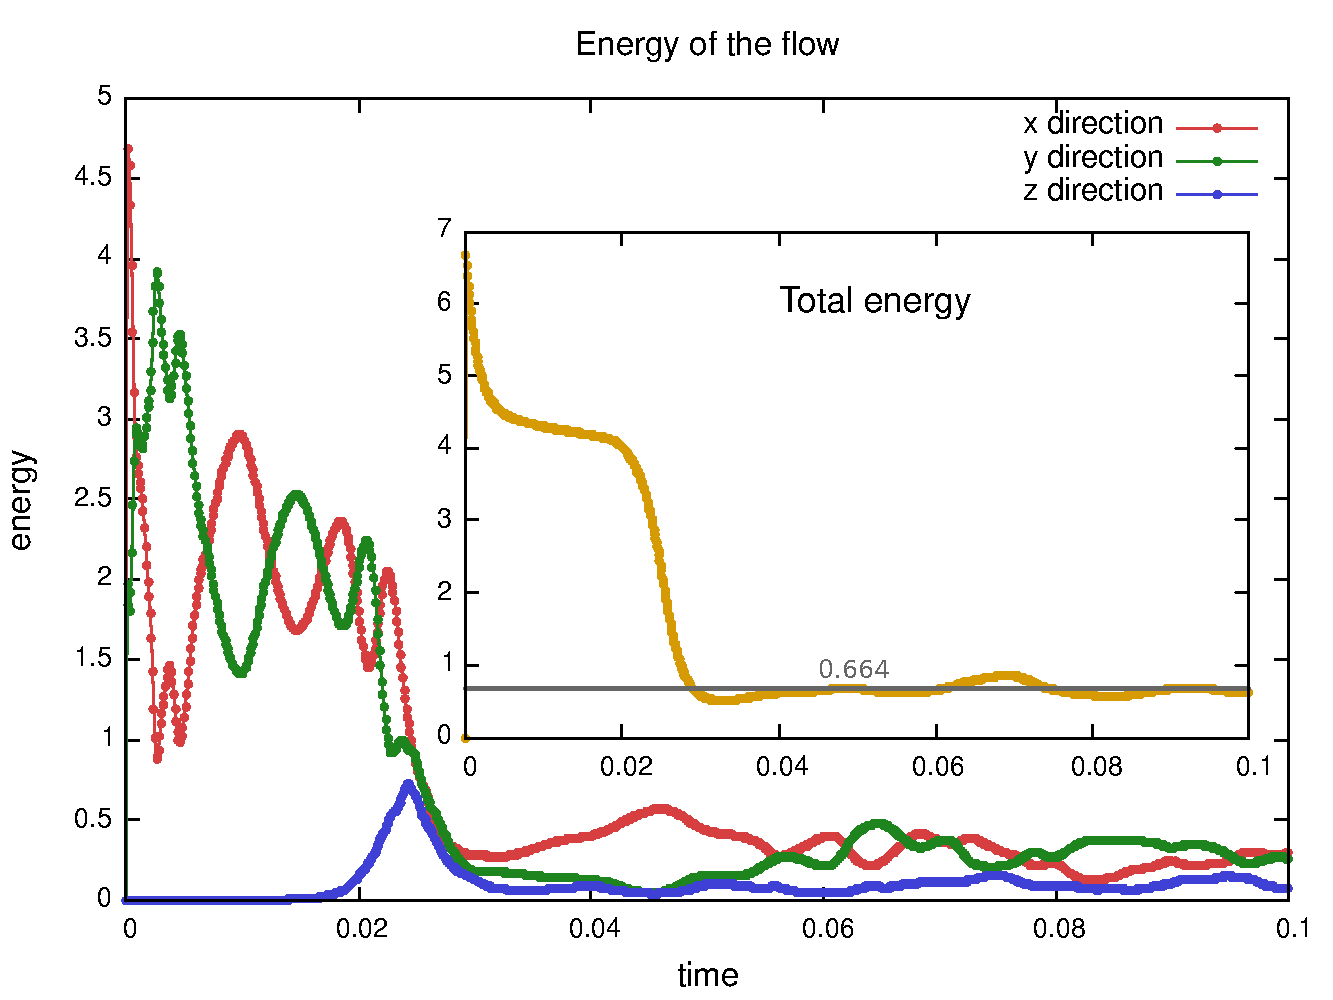
\includegraphics[width=\textwidth]{data/3D_model/thermalization/energy}
    \caption{The energy in function of time is represented: the horizontal directions dominate the total energy, which settles at a stable value.}
    \label{fig:therm_energy}
\end{figure}
    
\begin{figure}[ht]
    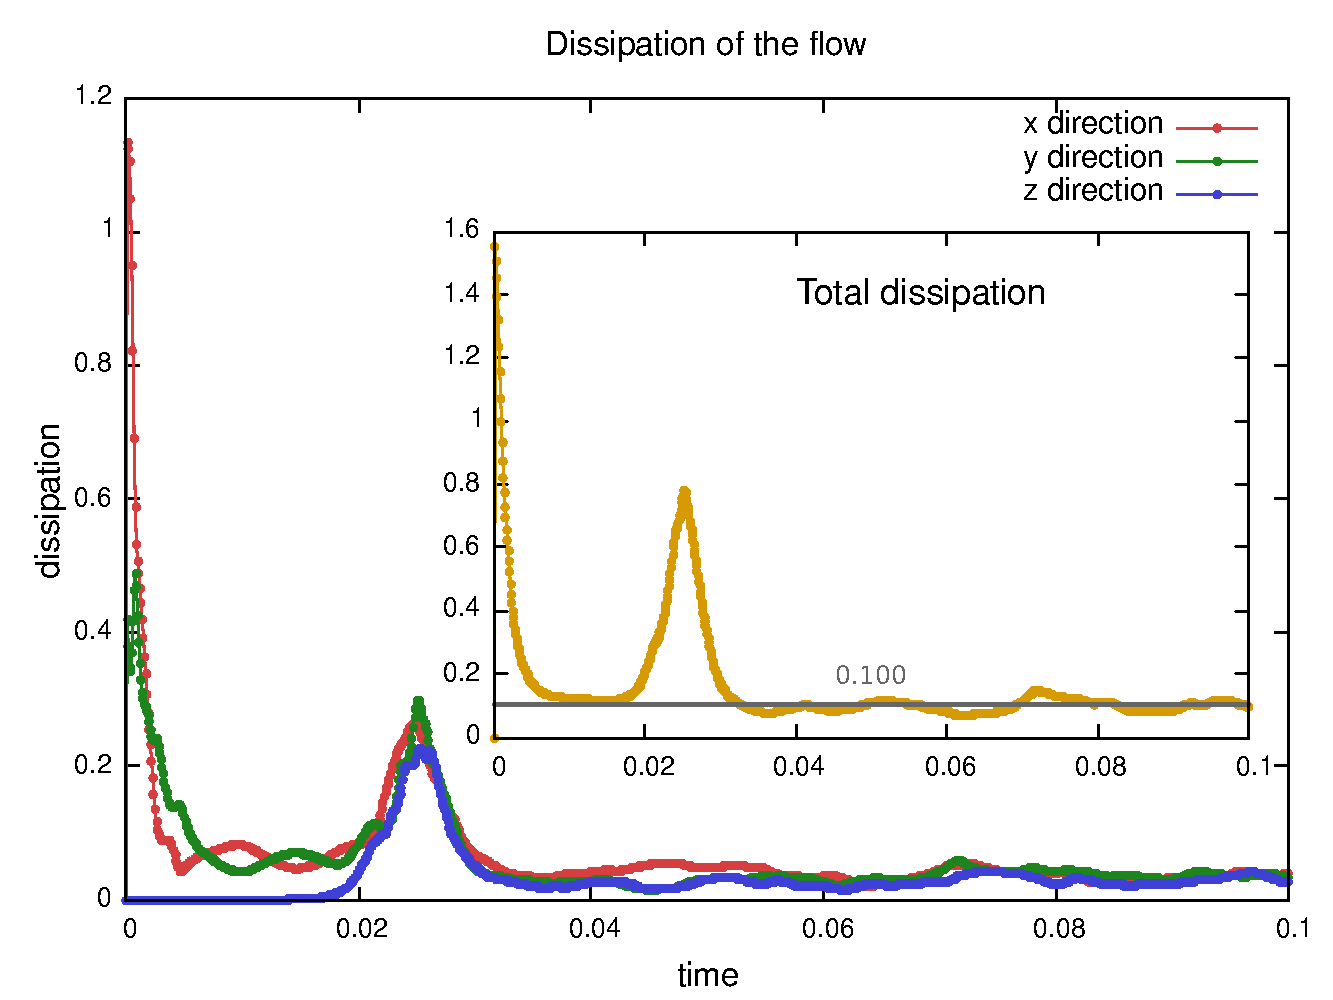
\includegraphics[width=\textwidth]{data/3D_model/thermalization/dissipation}
    \caption{The dissipation in function of time is represented: the horizontal directions dominate the total dissipation, which settles at a stable value.}
    \label{fig:therm_dissip}
\end{figure}
    
    
\subsubsection{Velocity field}
The resulting average squared velocities in function of depth are shown in \autoref{fig:vel_profile_xy} and \autoref{fig:vel_profile_z}. As seen above, the horizontal directions are dominant in magnitude. The no-slip boundary condition being imposed on the upper and lower boundaries, the vertical velocity must cancel there, and this feature is easily seen in \autoref{fig:vel_profile_z}.
    
\begin{figure} [ht]
    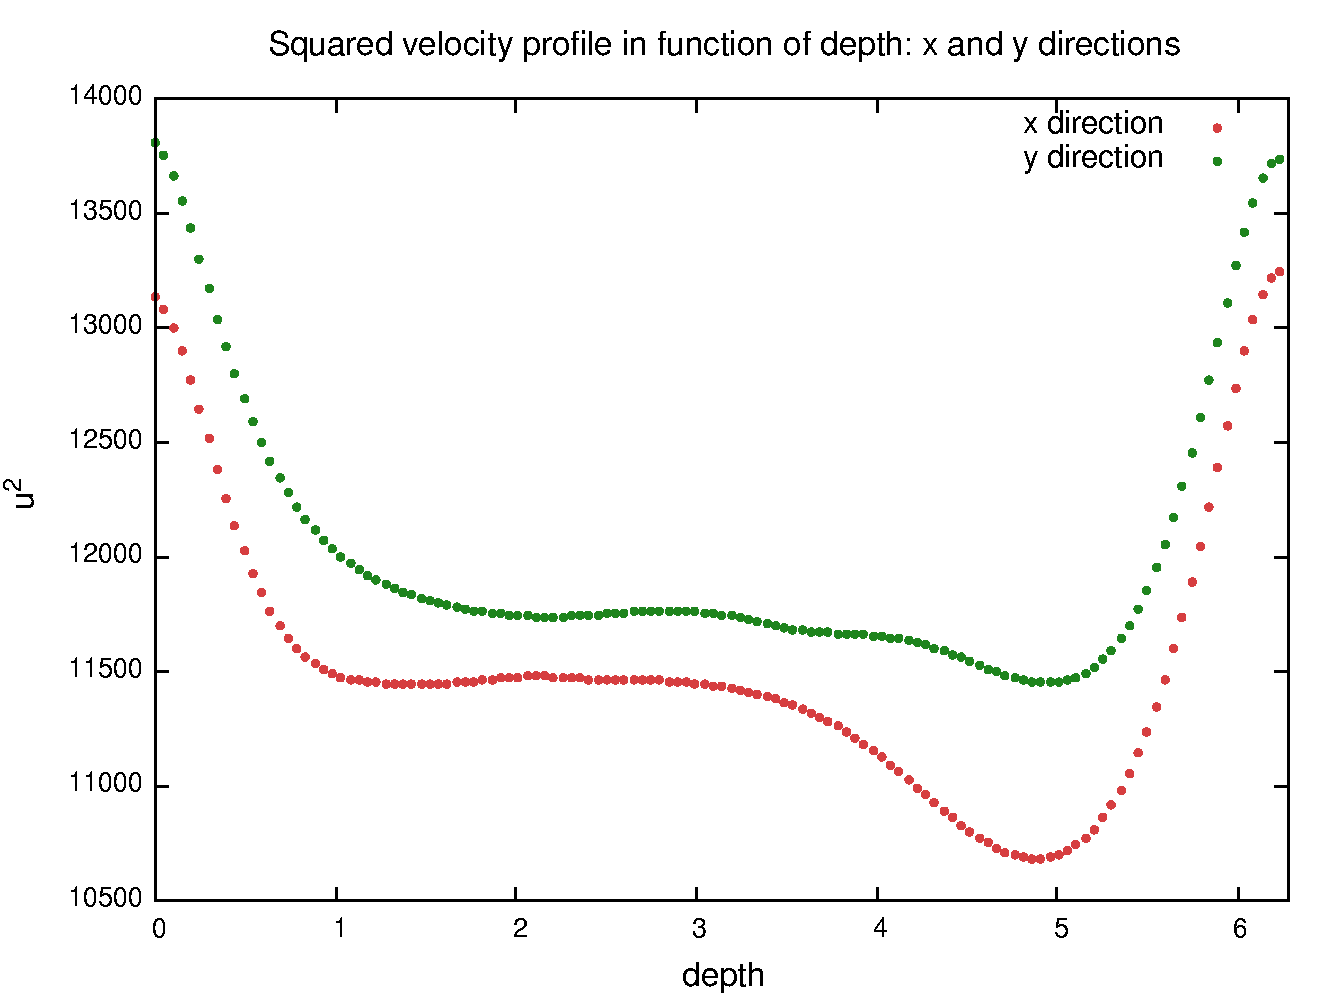
\includegraphics[width=\textwidth]{data/3D_model/run2/velocity_profile_xy}
    \caption{The profile of squared velocity along horizontal directions, averaged along horizontal planes.}
    \label{fig:vel_profile_xy}
\end{figure}

\begin{figure} [ht]
    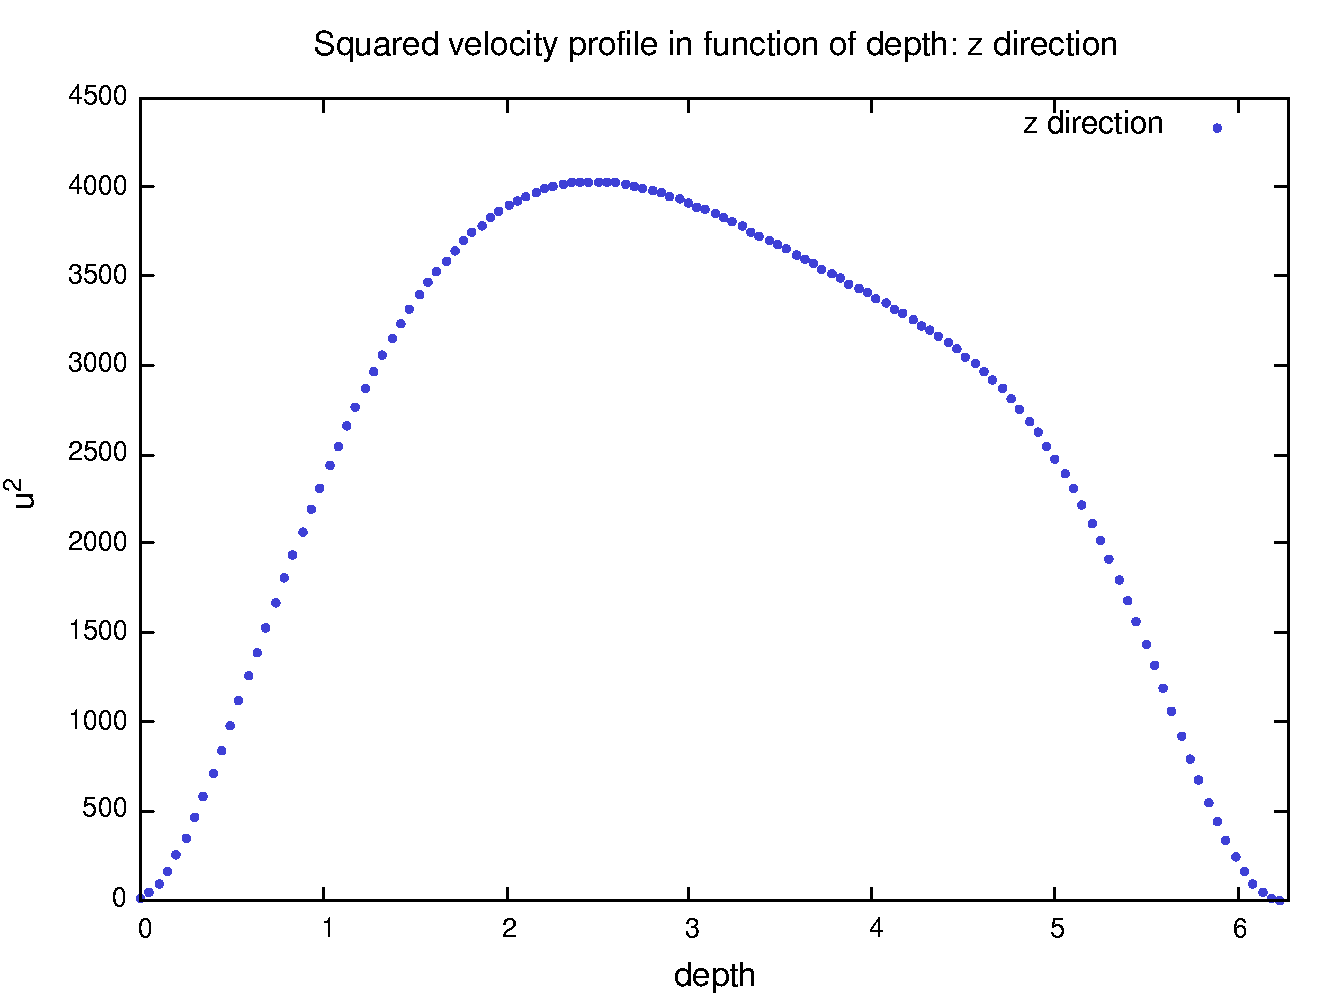
\includegraphics[width=\textwidth]{data/3D_model/run2/velocity_profile_z}
    \caption{The profile of squared velocity along the vertical direction, averaged along horizontal planes.}
    \label{fig:vel_profile_z}
\end{figure}

\subsection{Reaching the steady state} \label{sec:lag_steady}
In order to reach a steady state, it is necessary to have a saturation, which is granted by the self-shading effect in the model equation. However, when the sinking velocity is null, no steady state is reached. If no sink is present, the particles can remain longer in the bin at the top of the grid. The light intensity seen by a particle is the result of an interpolation between its values at the upper and lower grid points, and if a particle is in the top bin it will interpolate with the top grid point. This point, being above all particles, has a value of light intensity which is not attenuated by the shadowing of cells (the self-shading effect of the model). The result is that, no matter how many particles are present, they can always grow indefinitely if they remain near enough to the surface\footnote{This would not be the case if the particles had a finite volume, a feature not present in the model.}. %As can be seen in \autoref{fig:lag_res_novel_pop}, this leads to an uncontrolled growth. 
This effect makes the model not suitable to describe a neutrally or positively buoyant phytoplankton species.

%\begin{figure} [ht]
%    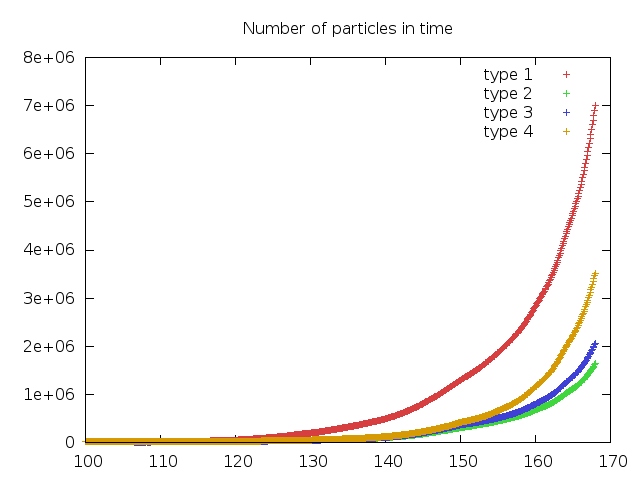
\includegraphics[width=\textwidth]{data/3D_model/run0/number}
%    \caption{The number of cells in function of time, with null sinking velocity. Four different populations are considered, with different $k_{ss}$, respectively $1.5\cdot10^{-4}$, $1.5$, $1.5\cdot10^4$, $1.5\cdot10^8$. The result confirms that the population grows indefinitely, despite changing the self-shading coefficient.}
%    \label{fig:lag_res_novel_pop}
%\end{figure}


\subsection{Effective diffusivity}
In order to evaluate the diffusivity, the method described in \autoref{sec:taylordiff} is used. %Since no steady-state is reached (see \autoref{sec:lag_steady}), the non-rigorous approach has to be undertaken, giving an indicative estimate of diffusivity. The time dependence is shown in \autoref{fig:lag_diff_novel}. After an initial transient phase, the values settle in a restricted interval, see the error in \autorefon interpolation.
In \autoref{tab:lag_res_diffu} the non-dimensional coefficient $C$ is calculated in correspondence either to the maximal velocity (simulation, see \autoref{sec:lag_res_number}) or to the minimal diffusivity (prediction and results in \autocite{Huisman2002HowPersist}), in order to compare the results with that model. 
%The compatibility is \( \Gamma_{A,B} = \left| \frac{ C_A - C_B}{\sqrt{\sigma_A^2+\sigma_B^2}} \right| \) and, despite of the name, estimates how much two results are incompatible \autocite[chapter 12.5]{loreti2006teoria}. At a first sight, the compatibility is very bad, the values of $C$ differing of more than one order of magnitude; introducing the compatibility, the situation gets a little better, at least when considering an error on the result by Huisman, obtained taking one half of the ticks spacing on the graph from which it has been read. \\
This result seems discouraging, but the two models are very different and no perfect match is to be expected. This result means that the two models just cannot be overlapped, while their qualitative outcomes are comparable.\\
Using the parameters in \autoref{tab:therm_values}, with the dimensional reasoning one finds $D=2$ and $C=0.03$, which is a worse estimate and will not be considered.

\begin{table}
    \centering
    \begin{tabular}{ c || c | c }
        & Simulation & Prediction \\
        \hline
        $D$
            & $9\cdot10^{-3}$ 
            & $1.5\cdot10^{-2}\,m^2h^{-1}$ \\
        $v$
            & $2.2\cdot10^{-2}$
            & $0.04\,mh^{-1}$ \\
        $k_{bg}$ 
            & $3.18$ 
            & $0.2\,mh^{-1}$ \\
        $C$ 
            & $0.07$ & $13$ \\   
        %\hline
        %$\Gamma$
        %    &  \multicolumn{2}{ c }{3.1}     \\
    \end{tabular}
    \caption{Comparison of results of the model with the theoretical value as seen in \autoref{sec:huism_crit_parameters}, by means of the non-dimensional parameter $C$ (\autoref{sec:adimensionalization}).} %For a definition of the compatibility $\Gamma$, see the text.}
    \label{tab:lag_res_diffu}
\end{table}

%\begin{figure} [H]
%    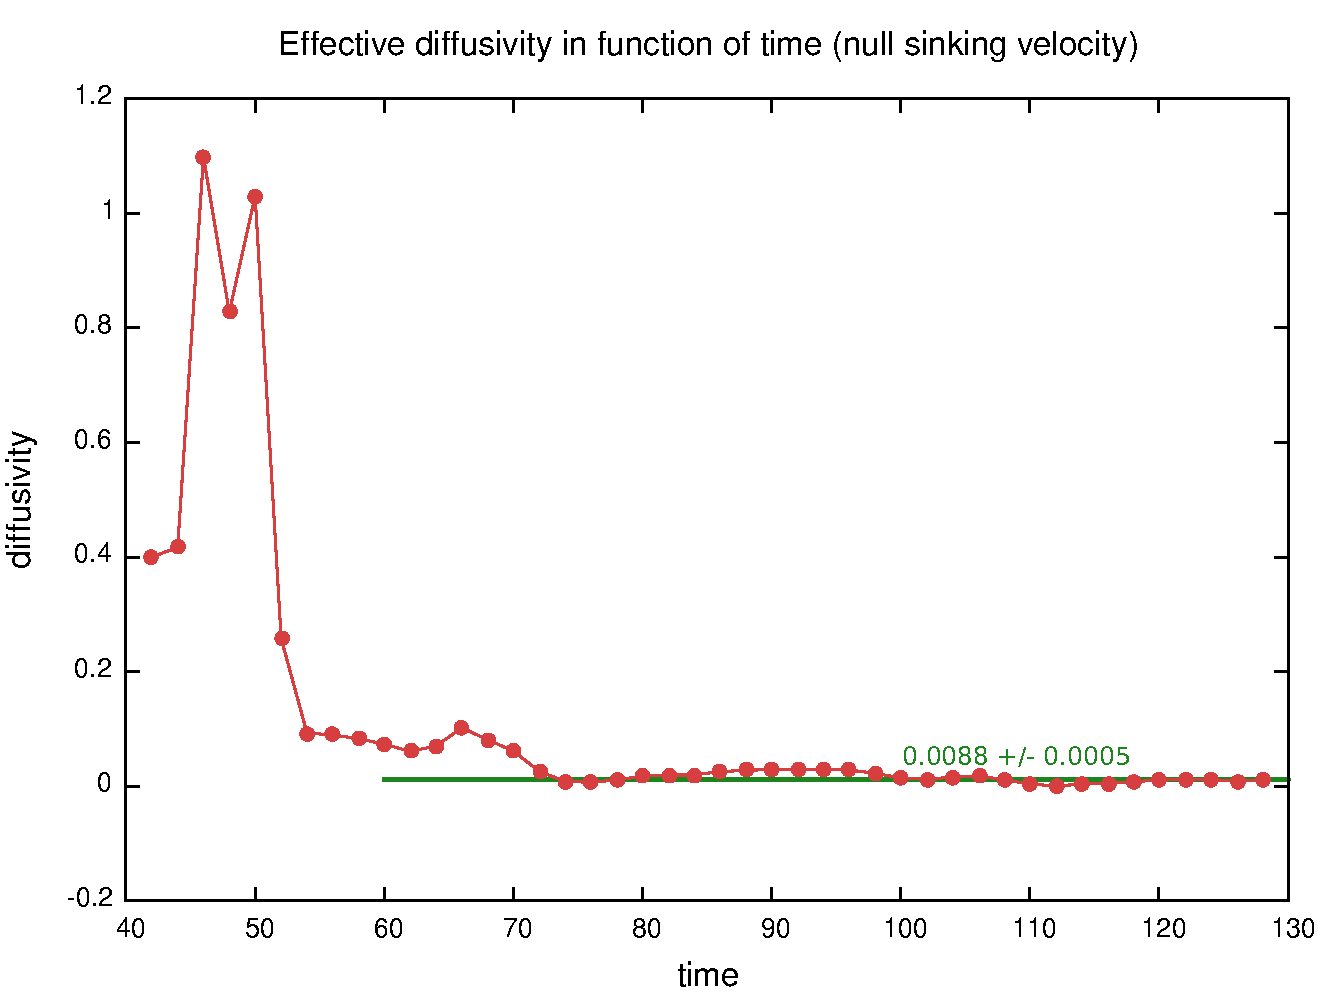
\includegraphics[width=\textwidth]{data/3D_model/run0_frequent/diffusivity}
%    \caption{Diffusivity evaluated as in \autoref{sec:taylordiff}, without reaching a steady-state.}
%    \label{fig:lag_diff_novel}
%\end{figure}

\begin{figure}[h]
        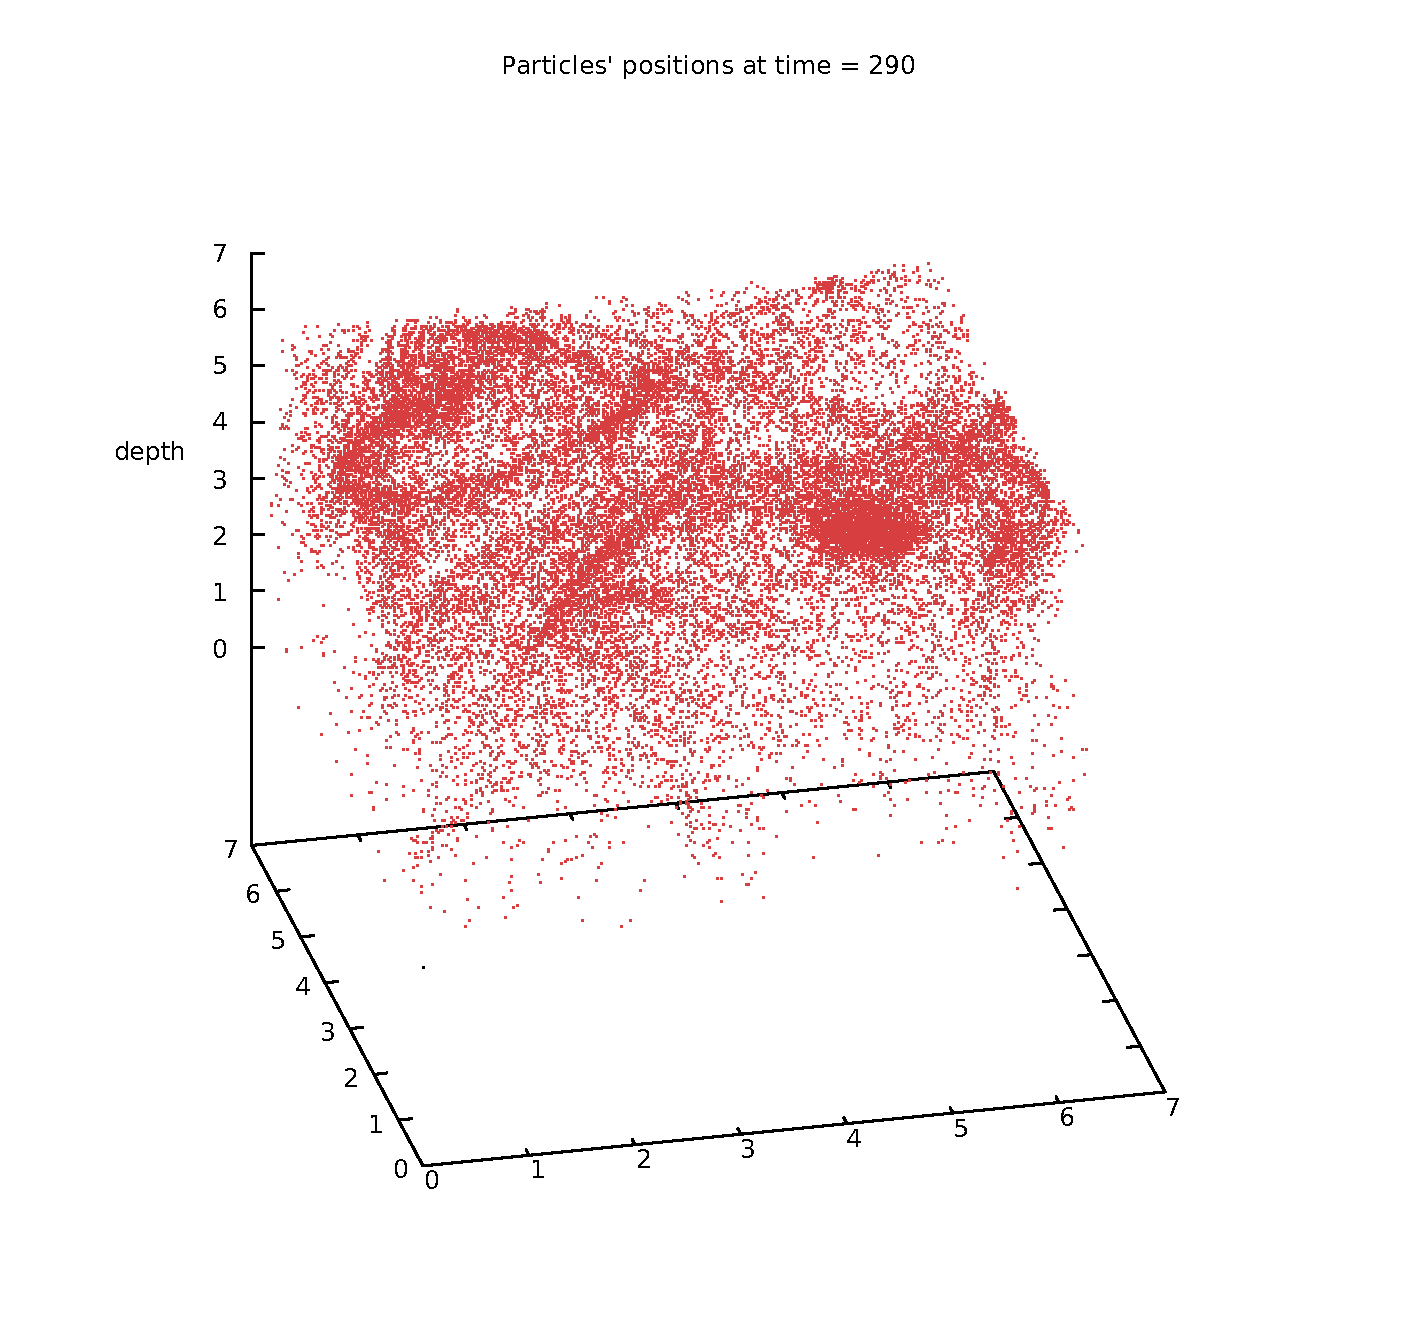
\includegraphics[width=\textwidth]{data/3D_model/run2/positions_145_1_C}
        \caption{A 3-dimensional view of the particles distribution.}
        \label{fig:lag_res_3D}
\end{figure}


\subsection{Distribution of particles} \label{sec:lag_res_distribution}


In \autoref{fig:lag_res_3D} a 3-dimensional configuration of the phytoplankton population has been plotted. In this section, the distribution over depth of the population, and its degree of non-randomness are discussed. It will turn out, as can be seen qualitatively, that there are indeed structures, not only in the vertical direction, but also horizontally.


\begin{figure}[ht]  
    \begin{subfigure}[b]{0.68\textwidth}
        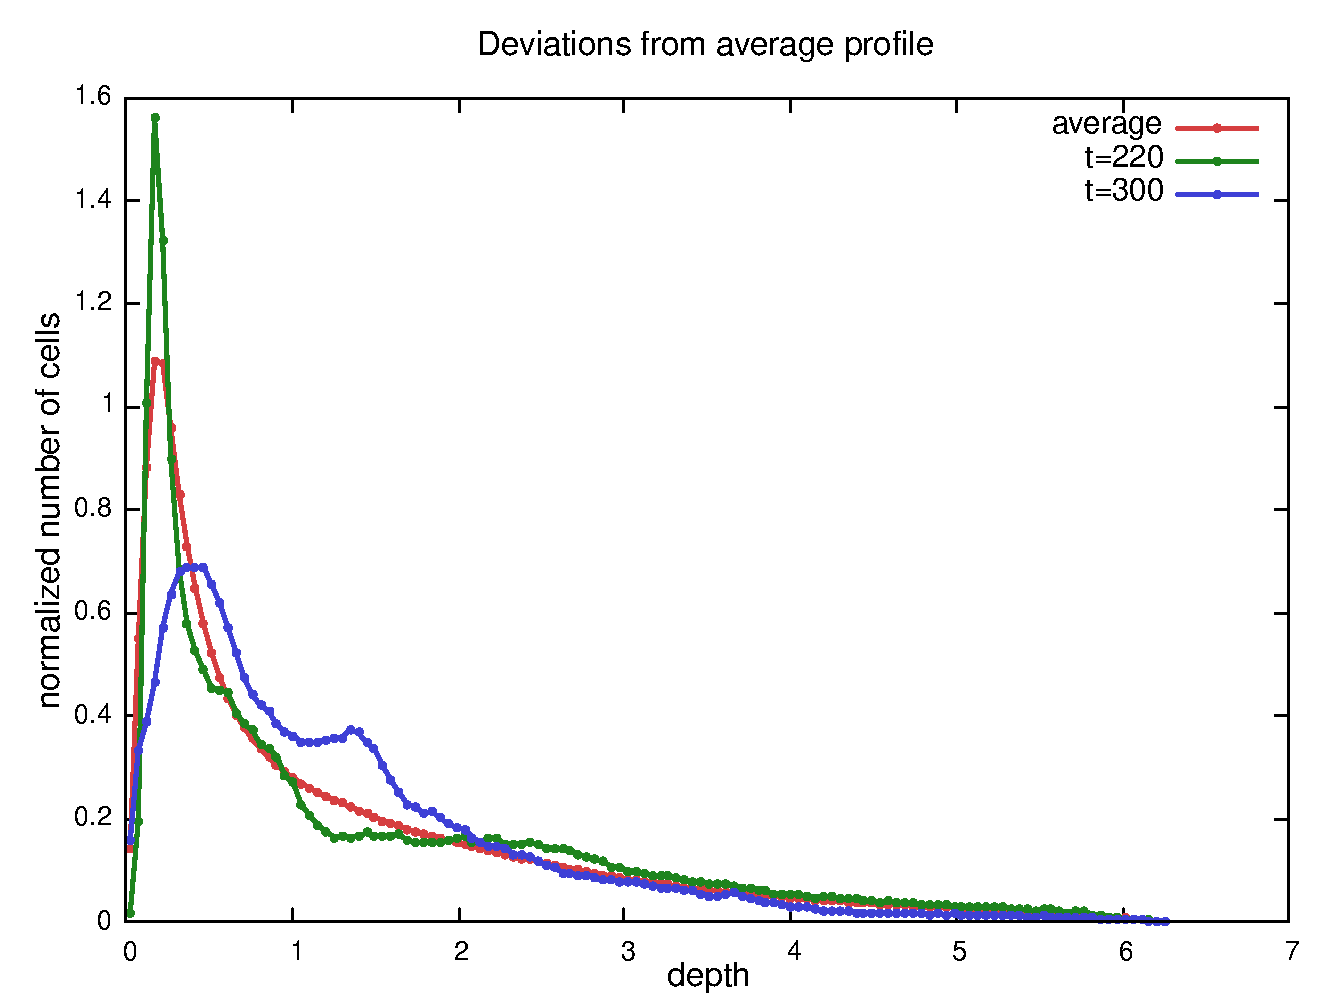
\includegraphics[width=\textwidth]{data/3D_model/run2/profile_deviation}
        \caption{}
        \label{fig:lag_res_prof_deviation_profile}
    \end{subfigure}
    \begin{subfigure}[b]{0.3\textwidth}
        \begin{minipage}[t]{\linewidth}
        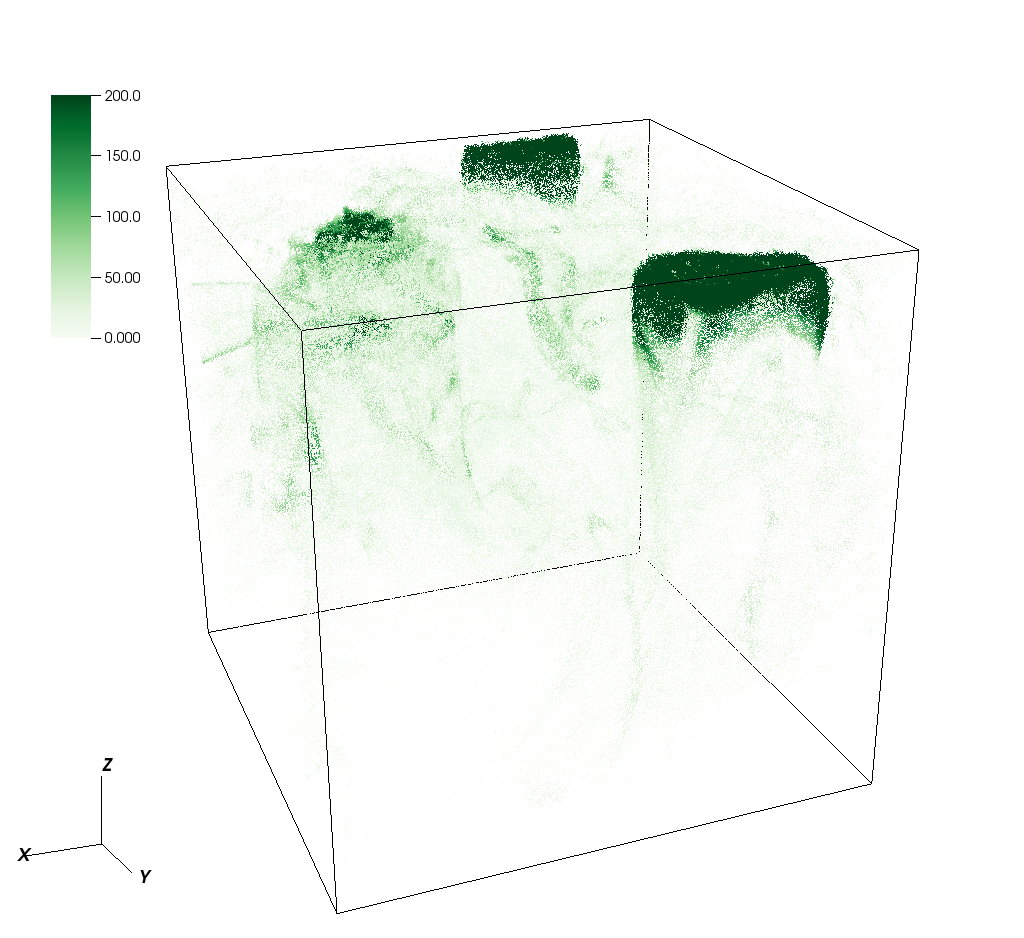
\includegraphics[width=\textwidth]{data/3D_model/run2/positions_110_coloured}
        \end{minipage} \quad
        \begin{minipage}[t]{\linewidth}
        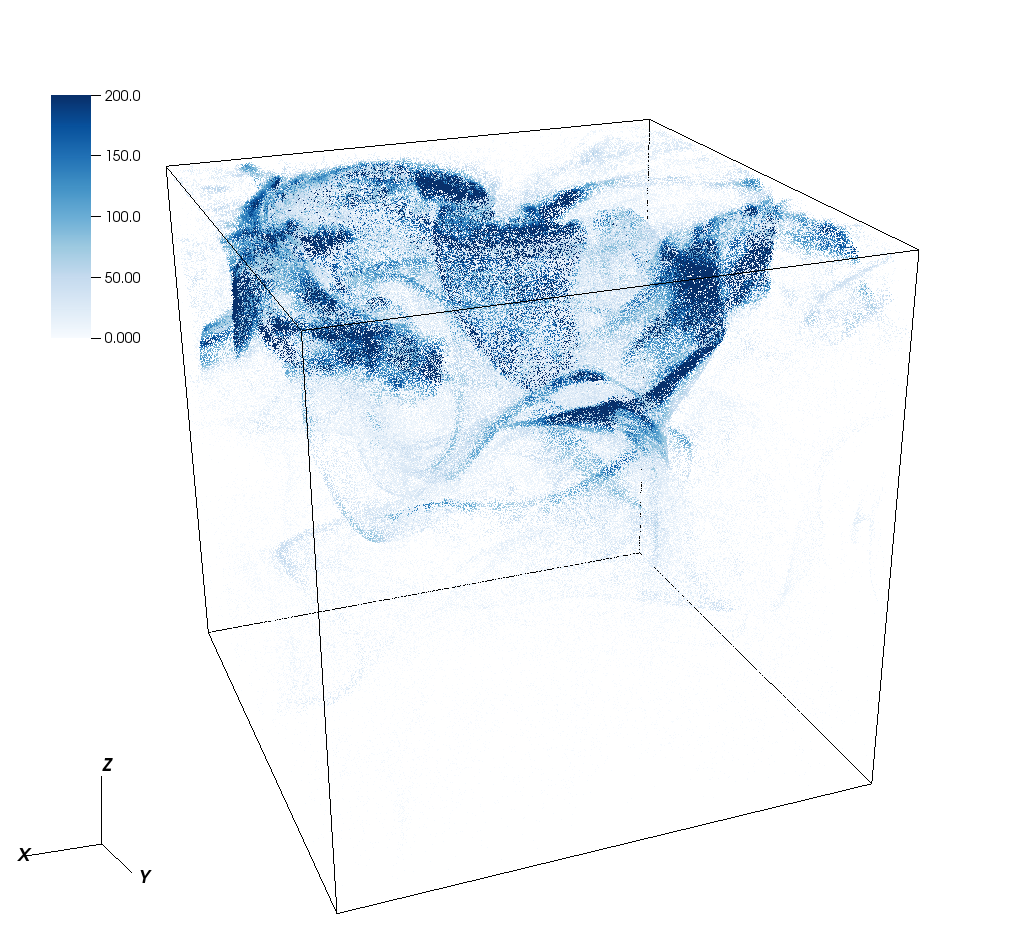
\includegraphics[width=\textwidth]{data/3D_model/run2/positions_150_coloured}
        \end{minipage}
        \caption{}
        \label{fig:lag_res_prof_deviation_3D}
    \end{subfigure}
    \caption{In \autoref{fig:lag_res_prof_deviation_profile}: depth profile deviations from the average over time. Two times at which the profile deviates much from the average have been selected When the steady state is reached, the values oscillate around a stable value. In \autoref{fig:lag_res_prof_deviation_3D}: 3-dimensional distribution of cells for the two deviating profiles (colours match), where the palette saturates at 200, for sake of clarity, but the maximum value reaches respectively 1930 and 2154 for times 220 and 300.}
    \label{fig:lag_res_prof_deviation}
\end{figure}

\subsubsection{Depth profile} \label{sec:lag_res_profile}
Of qualitative interest is the shape of the depth profile $\rho(z_i,t_i)$ of the population: it is obtained making an histogram with the positions of the particles along the vertical axis, $z_i$ representing the value of distance from the bottom at the bin $i$, and $t_i$ being a discrete time at which the profile is considered. It is in principle time-dependent. \\
The result resembles that of \autoref{sec:stoc_res_profile}, having a peak under the surface and decaying towards the bottom. An average over time can be seen in \autoref{fig:lag_res_prof_deviation}, as well as two snapshots at specific times are compared with it. A characteristic feature is a second peak, deeper than the first one, which appears and disappears with time and may be a plume detaching from the bulk under the surface. This is coherent with the observation of plumes under the surface when looking at the 3-dimensional distribution (\autoref{fig:lag_res_prof_deviation_3D}); further analysis is however needed to confirm this hypothesis. 



Looking for a more quantitative approach to the evolution of the profile shape, in \autoref{fig:lag_res_rho_err} the profile is averaged over time
\[ \langle \rho \rangle \coloneqq \frac{\sum_{\{t_i\}} \rho(t)}{\Delta t} \]
The plot shows a reasonably small deviation from the mean, backing up the claim that the shape does not change much during the simulation.%; a further confirmation comes from considering the evolution in time of the following estimator $s$ of the error at a given time:
\[ s(t_i) = \frac{\sum_{\{z_i\}} \left| \rho(z_i,t_i) - \langle \rho \rangle(z_i) \right|}{N_{bins}} \]
%In \autoref{fig:lag_res_rho_err_time} the evolution of $s$ in time is displayed, showing a rather constant behaviour over time, randomly scattered around an average value. \\
Considering how the number of particles varies in time (see \autoref{sec:lag_res_number}) two main phases can be identified: the first one corresponds to an exponential growth, while the second one is a dynamical equilibrium oscillating around a central value. It is interesting to look at how the shape of the profile changes between these two phases, and a graphical comparison is in \autoref{fig:lag_res_rho_comparison}: when the quasi-steady state is reached, the peak is less pronounced, with a more consistent tail. The following interpretation is proposed: when the growth is exponential, the diffusive-advective processes (flow transport and sink; see \autoref{sec:lag_part_adv}) are not fast enough to spread the peak with respect to the birth processes; when instead the self-shading effect effectively limits the population growth rate, these spreading effects can play a substantial role, resulting in a longer tail. 

\begin{figure}[ht]
    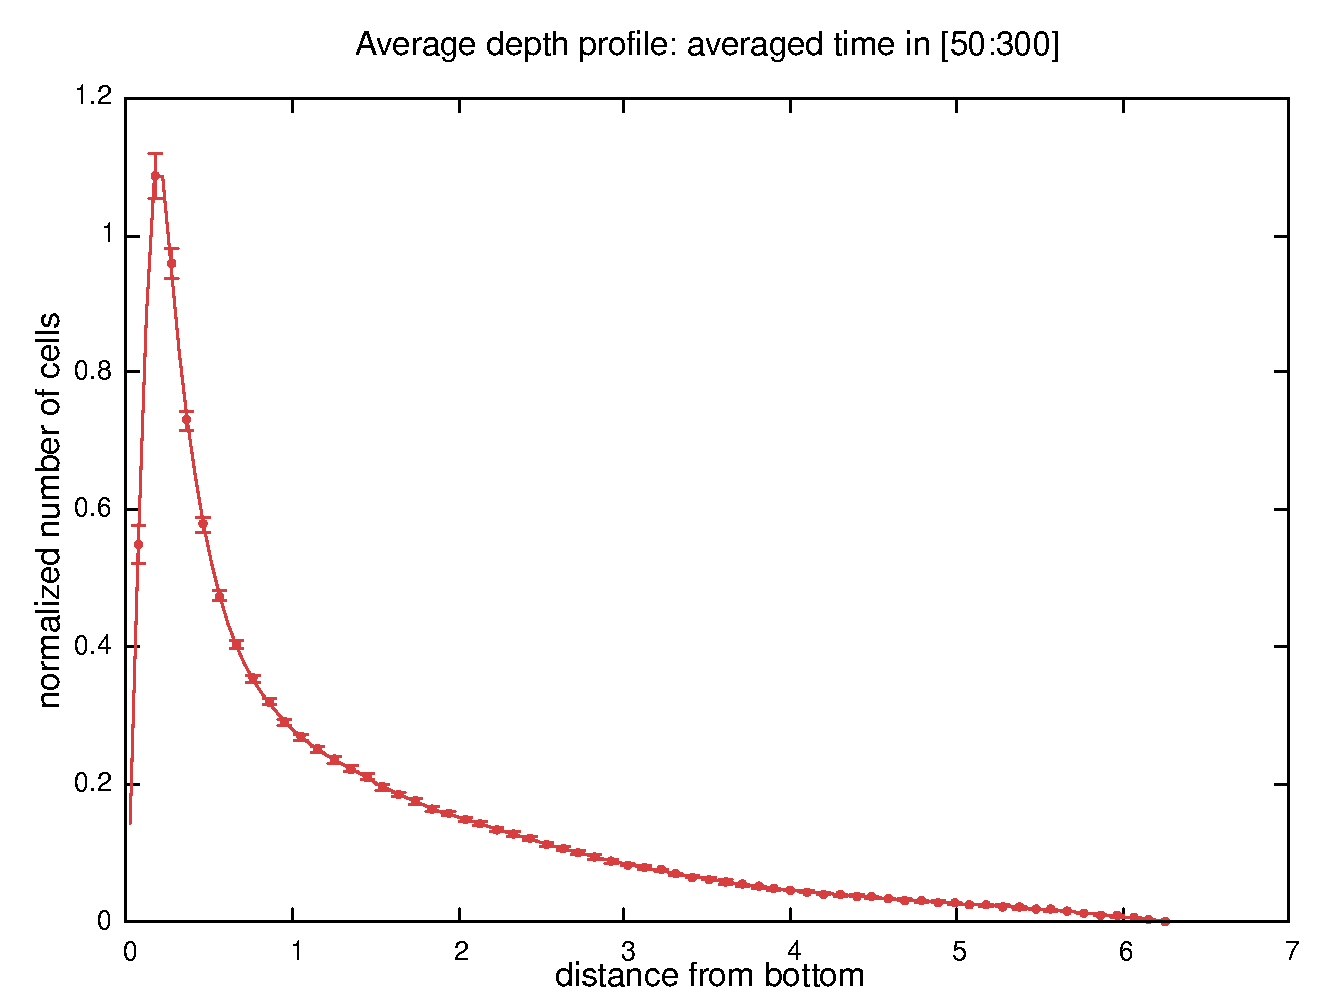
\includegraphics[width=\textwidth]{data/3D_model/run2/profile_avg_1_50_300}
    \caption{Averaged depth profile, in the steady phase.}
    \label{fig:lag_res_rho_err} \label{fig:lag_res_prof_err}
\end{figure}

\begin{figure}[h]
        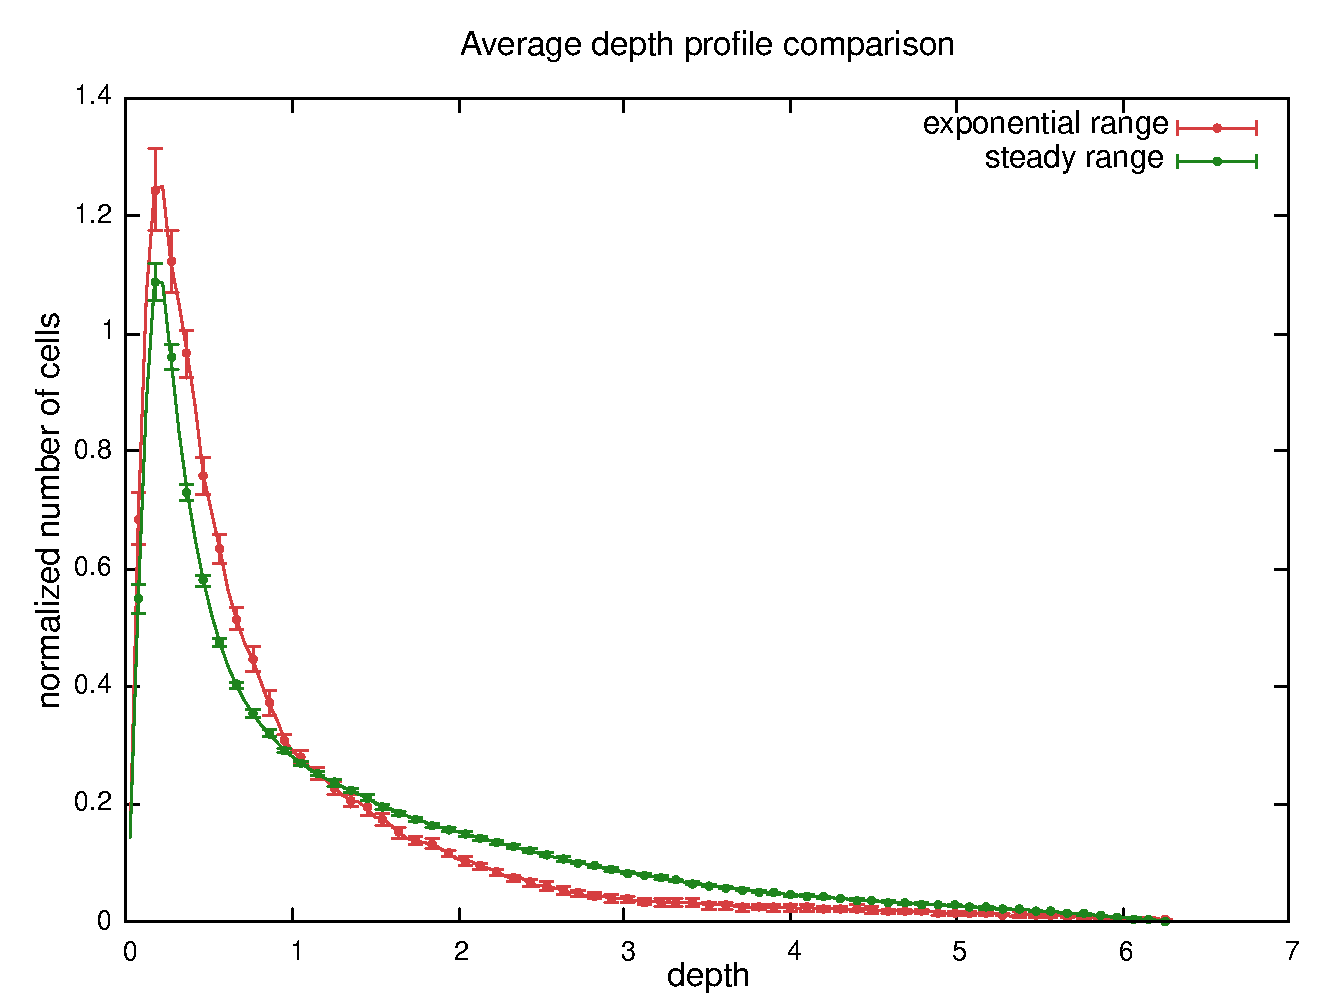
\includegraphics[width=\textwidth]{data/3D_model/run2/rho_comparison}
        \caption{The average profile during and after the exponential range (see \autoref{sec:lag_res_number}).}
        \label{fig:lag_res_rho_comparison}
\end{figure}


\subsubsection{Randomnesss} \label{sec:lag_res_random}
In order to quantitatively detect the patchiness present in the spatial distribution of the cells, a meaningful quantity which can be defined is the \textit{deviation between mean and variance}, which is an estimator of the deviation from randomness. The Poisson distribution is \autocite[chapter 8.5]{loreti2006teoria}
\[ P(x;\lambda) = \frac{e^\lambda \lambda^{-x}}{x!} \]
and its mean $\mu$ and variance $\sigma^2$ are
\[ \mu = \sigma^2 = \lambda \]
This distribution models rare, random events occurrence. Evaluating the relative difference between these two values relative to the mean gives an estimate of the deviation from the Poisson distribution, and thus from randomness. \\
For an analysis of the simulated structure, the particles have been grouped in ``boxes'' of varying size, then the number of particles in each box has been sampled, and put in a histogram which looks at the distribution of the number of particles per box along the vertical direction.
The results can be seen in \autoref{fig:lag_res_random}: the binning on vertical direction is kept constant, in order to notice the horizontal clustering structure. While increasing the dimension of horizontal bins, the deviation from randomness accentuate, to reach a maximum at $\sim\frac{1}{3}$ of the simulation box size, and then decrease. When the binning is very dense, the boxes probe a length which is too small to detect structure; on the contrary, when the binning reaches a size similar to the simulation box, the irregularities are averaged out. This means that the characteristic size of the patches is comparable to the binning size of the higher curve, that is, approximately a third of the side length. 

\begin{figure}[h]
    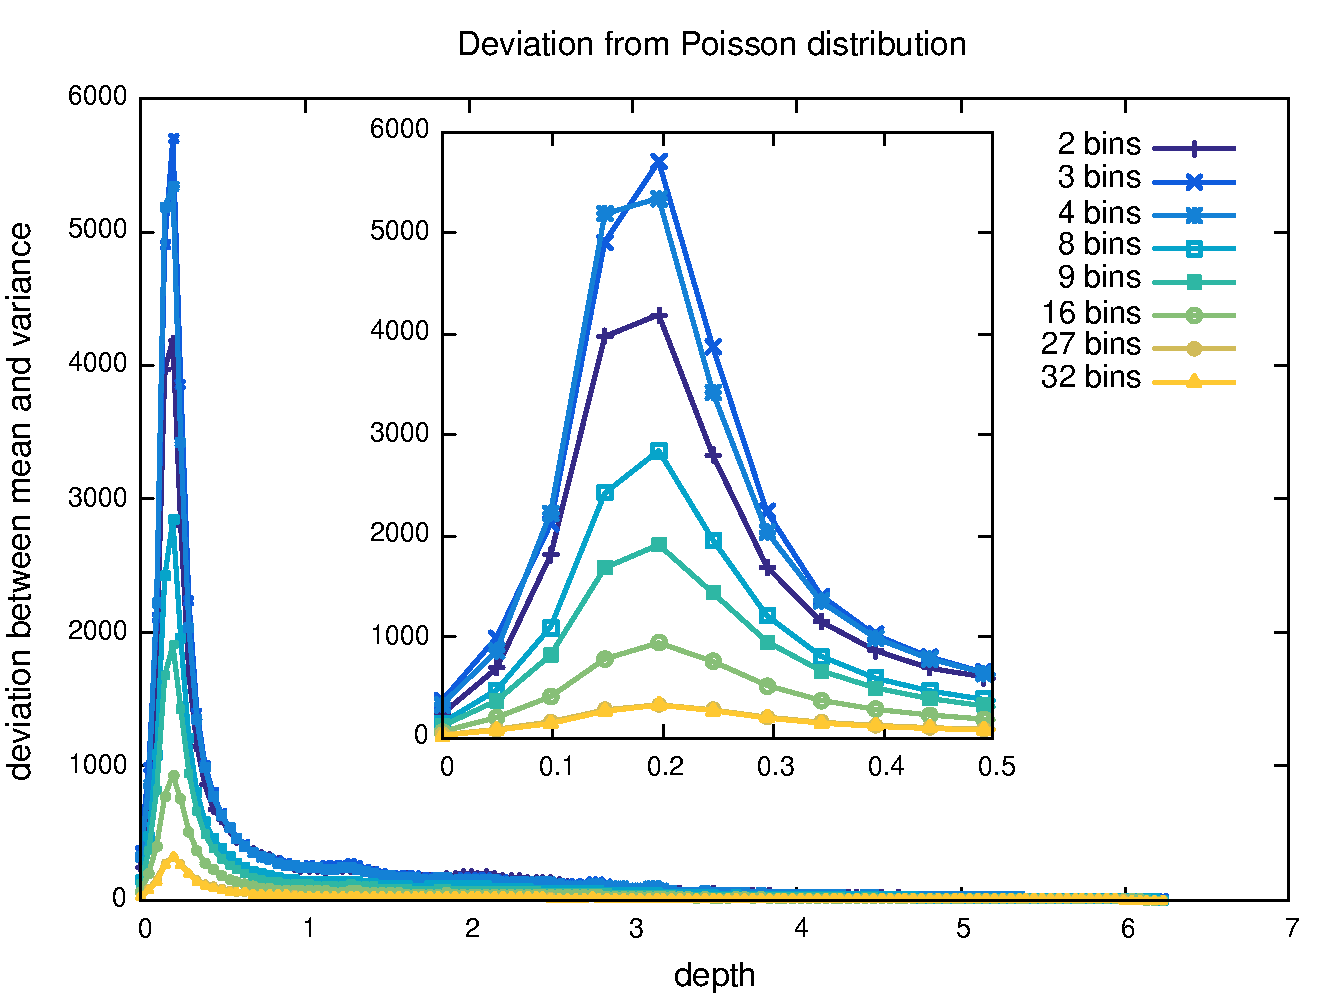
\includegraphics[width=\textwidth]{data/3D_model/run2/dev_poisson_1}
    \caption{The relative difference between mean and variance for the particles distribution at different binnings in the horizontal directions. The deviation from Poisson's distribution increases while increasing the bin size, having a maximum at $\sim\frac{1}{3}$ of the simulation box and then decreasing.}
    \label{fig:lag_res_random}
\end{figure}



\subsection{Number of particles} \label{sec:lag_res_number}
In \autoref{fig:lagr_v0_k0_number} the number of cells in function of time is plotted, showing an exponential transient phase, interpreted as the phase in which the self-shading effect is not large enough to damp growth. In \autoref{fig:lagr_v0_k0_number_zoom}, this transient phase is enlarged and fitted with an exponential function, whose values are shown in \autoref{tab:fit_number}. The third value shown is the prediction for the logarithmic slope made with the following reasoning. Writing \( n(z,t) = N(t) \rho(z,t) \) one can isolate the shape $\rho$ of the profile from its integral, imposing \( \int_L \rho(z,t) \dd z \equiv 1 \) with $L$ the total length of the water column. It follows that the equation \( \partial_t n(z,t) = g(z) n(z,t) \), where the self-shading effect is neglected, thus $g$ is constant in time, becomes
\[ \partial_t N(t) = N(t) \int_L g(z) \rho(z,t) \dd z \]
having as a solution
\[ N(t) = N_0e^{ \int_L g(x) \rho(z,t) \dd z \dt } \]
which if $\rho(z,t) \sim \rho(z)$ (see \autoref{fig:lag_res_prof_err}) becomes
\[ N(t) = N_0 e^{ \langle g\rangle t} \]
where the angled brackets mean a spatial average weighted with the unitary density $\rho$.

\begin{table}
    \centering
    \begin{tabular}{ c || c c | c || c}
        interval & $A$ & $k$  &  $\langle g \rho \rangle $ & $\left| \frac{k - \langle g \rho \rangle}{\sqrt{\mathrm{var}(k)+\mathrm{var}(\langle g \rho \rangle)}} \right|$ \\
        \hline 
        %$[10,25]$ & $4800\pm100$ & $0.096\pm0.001$ & $0.12\pm0.03$ & $0.80$ \\
        %$[25,50]$ & $9000\pm100$ & $0.0754\pm0.0003$ & $0.07\pm0.02$ & $0.26$ \\
        $[10,50]$ & $8100\pm100$ & $0.0777\pm0.0003$ & $0.09\pm0.02$ & $0.61$ \\
    \end{tabular}
    \caption{The parameters resulting from a fit of \autoref{fig:lagr_v0_k0_number_zoom} with the function $Ae^{kx}$ and the estimate of $k$ as the weighted average of the growth function $g$ over the profile. The fit is made with Gnuplot (\url{http://gnuplot.info/}).. Two different intervals are considered to take into account the variability of the coefficient.}
    \label{tab:fit_number}
\end{table}

\begin{figure}[h]
    \centering  
    \begin{subfigure}[b]{\textwidth}
        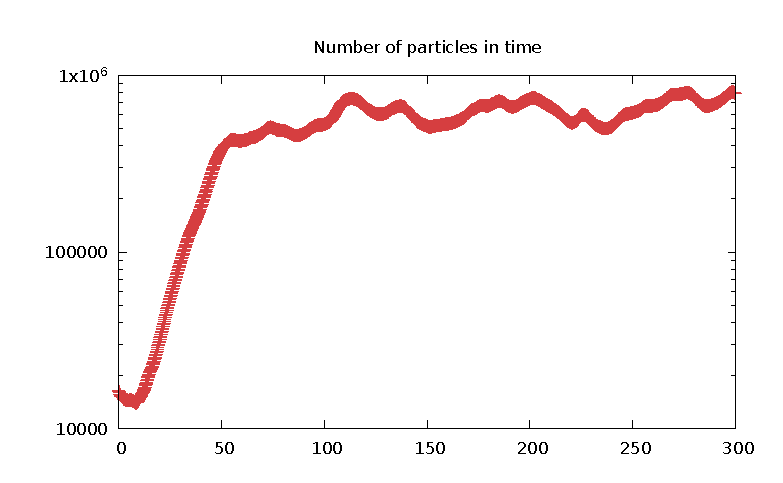
\includegraphics[width=\textwidth]{data/3D_model/run2/number_type1_log}
        \caption{}
        \label{fig:lagr_v0_k0_number}
    \end{subfigure}
    \begin{subfigure}[b]{\textwidth}
        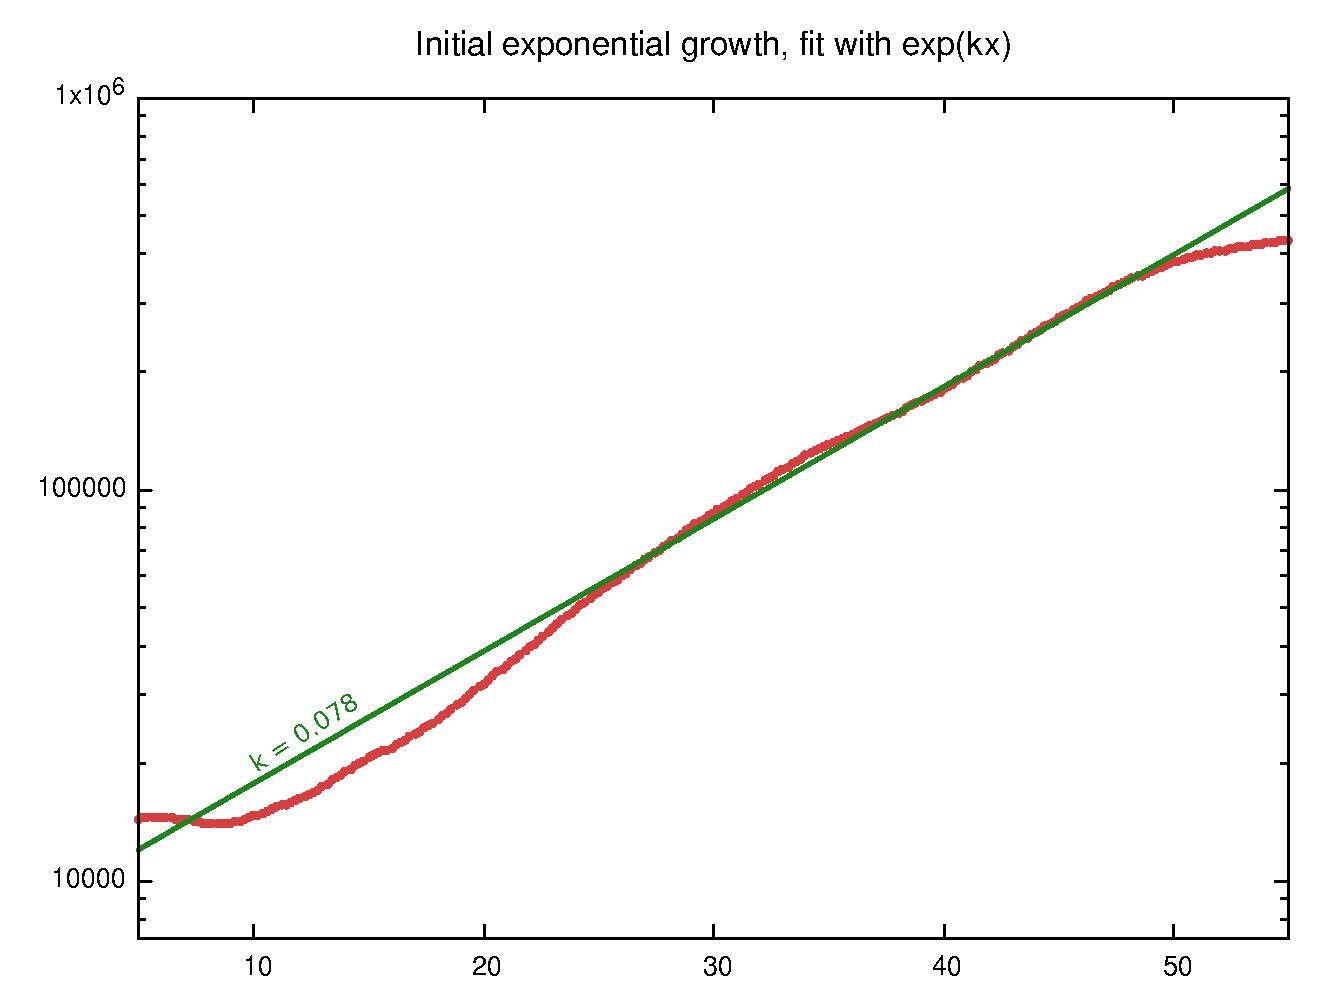
\includegraphics[width=\textwidth]{data/3D_model/run2/number_type1_log_zoom}
        \caption{}
        \label{fig:lagr_v0_k0_number_zoom}
    \end{subfigure}
    \caption{The particle number in function of time, and a closer view of the exponential growth which happens at the beginning of the simulation.}
    \label{fig:lagr_v0_k0_numbers}
\end{figure}

In \autoref{fig:lag_res_number}, the number of cells of three independent populations are plotted in function of time. The velocity changes from population to population, the other parameters being equal; this allows to measure a critical speed, defined as the average of the two higher speeds.

\begin{figure}[h]
    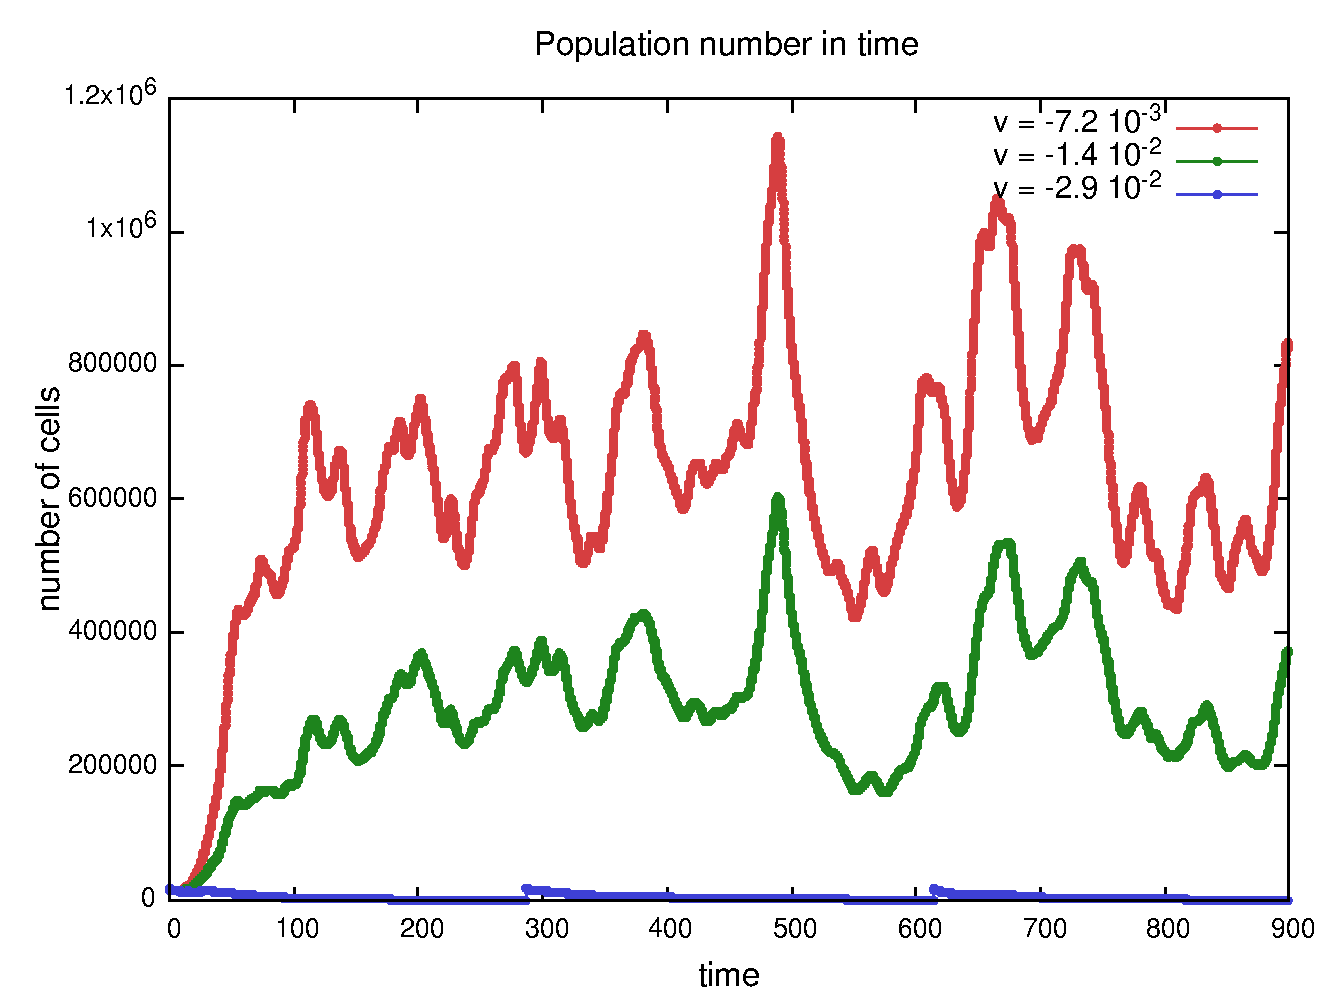
\includegraphics[width=\textwidth]{data/3D_model/run2/number}
    \caption{The number of particles in function of time for three different and non-interacting population. The characteristic growth time is \(\frac{1}{\mu} \sim 10\). The third type of cells is regenerated when the population dies off.}
    \label{fig:lag_res_number}
\end{figure}